\chapter{The Nintendo Switch and the Fusee Gelee Exploit}
\epigraph{quote}{\textit{author}}

\section{Nintendo Switch Security Overview}

\subsection{Security Architecture of the Nintendo Switch}

The Nintendo Switch, a popular gaming console, employs a multi-layered security architecture designed to protect both the hardware and software from unauthorized access and tampering. Central to this architecture is the use of a secure boot process, which ensures that only authenticated firmware and software can be executed on the device. The console utilizes several security mechanisms including ARM TrustZone, a security co-processor, and a microkernel with a modular, minimally-privileged architecture.

\subsection{The Role of Boot ROM and Secure Boot Process}

The Boot ROM is an essential component of the Switch's security architecture. It contains the initial code that is executed when the console is powered on. This code performs the critical task of verifying the integrity and authenticity of the subsequent stages of the boot process through cryptographic checks. The secure boot process involves several steps:

\begin{itemize}
    \item \textbf{ROM Code Execution}: The immutable Boot ROM code is executed first. This code is hardwired into the chip and cannot be modified post-manufacturing.
    \item \textbf{Verification of Bootloader}: The Boot ROM verifies the digital signature of the bootloader stored in non-volatile memory.
    \item \textbf{Loading and Executing Bootloader}: Upon successful verification, the bootloader is loaded into memory and executed, which in turn verifies and loads the operating system kernel.
\end{itemize}

This chain of trust is designed to prevent unauthorized code from running on the device, thereby protecting the system from low-level attacks.

\section{Discovery of Fusee Gelee Exploit}

\subsection{Technical Specifics of the Vulnerability}

The Fusee Gelee exploit, discovered by the hacking team ReSwitched, leverages a critical vulnerability in the Nvidia Tegra X1 chip used in the Nintendo Switch. The exploit targets a flaw in the USB recovery mode of the Tegra chip. Specifically, the vulnerability arises from an unchecked buffer during the handling of USB control transfers in the Boot ROM code\cite{roussel-tarbouriechMethodicallyDefeatingNintendo2019}\cite{WaybackMachine2019}.

When a device enters USB recovery mode, it expects a specific sequence of USB packets. The vulnerability is triggered by sending an oversized control transfer, which overflows a buffer in the Boot ROM, allowing the attacker to execute arbitrary code. This type of vulnerability is known as a buffer overflow attack\cite{BufferOverflow2024}.

\begin{minted}[frame=single, linenos, breaklines]{c}
    // If this is a warmboot (from "sleep"), restore the saved state from RAM.
    if (read_scratch0_bit(1)) {
      restore_warmboot_image(&load_addr);
    }
    // Otherwise, bootstrap the processor.
    else
    {
      // Allow recovery mode to be forced by a PMC scratch bit or physical straps.
      force_recovery = check_for_rcm_straps() || read_scratch0_bit(2);
    
      // Determine whether to use USB2 or USB3 for RCM.
      determine_rcm_usb_version(&usb_version);
      usb_ops = set_up_usb_ops(usb_version);
      usb_ops->initialize();
    
      // If we're not forcing recovery, attempt to load an image from boot media.
      if (!force_recovery)
      {
        // If we succeeded, don't fall back into recovery mode.
        if (read_boot_configuration_and_images(&load_addr) == SUCCESS) {
          goto boot_complete;
        }
      }
    
      // In all other conditions
      if (read_boot_images_via_usb_rcm(<snip>, &load_addr) != SUCCESS) {
         /* load address is poisoned here */
      }
    }
    
    boot_complete:
      /* apply lock-outs, and boot the program at address load_address */
\end{minted}
\captionof{lstlisting}{Tegra boot process approximation from\cite{WaybackMachine2019}}

\subsection{Exploitation Mechanism}

The exploitation process involves several steps:

\begin{itemize}
    \item \textbf{Initiating Recovery Mode}: The attacker forces the Switch into USB recovery mode by shorting specific pins on the right Joy-Con connector, which triggers the device to await USB communication.
    \item \textbf{Sending Malicious USB Payload}: A specially crafted USB payload is sent to the device. This payload is designed to overflow the buffer and overwrite critical memory regions.
    \item \textbf{Executing Arbitrary Code}: The overwritten memory regions include the instruction pointer, which is redirected to execute the attacker's payload. This payload typically includes a custom bootloader or code to bypass security checks.
\end{itemize} 

\begin{figure}[H]
    \centering
    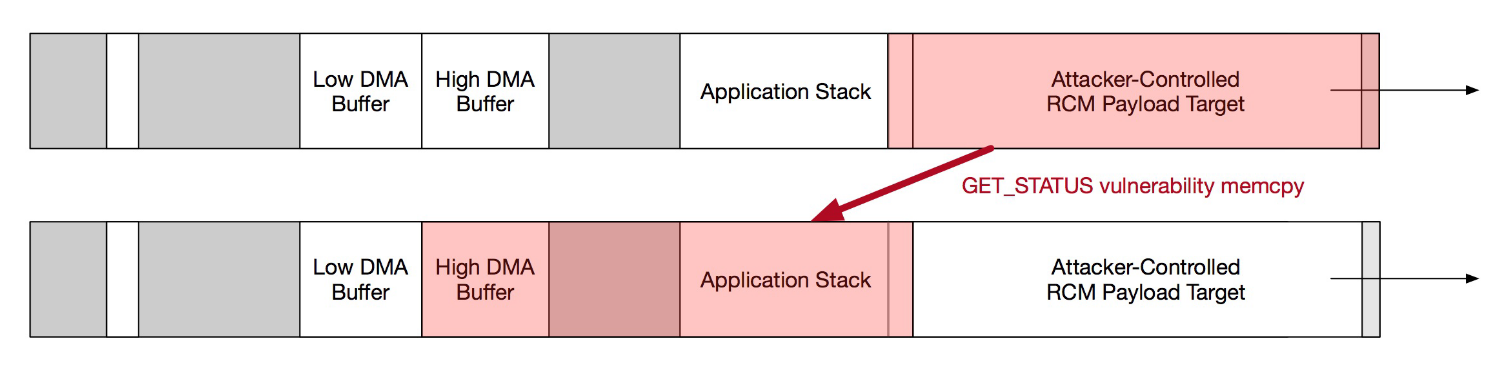
\includegraphics[width=0.9\textwidth]{images/overflow.png}
    \caption{Tegra X1 Boot ROM Buffer Overflow Exploit diagram from\cite{WaybackMachine2019}}
    \label{fig:fusee_gelee_exploit}
\end{figure}

The execution of arbitrary code at such an early stage of the boot process effectively allows the attacker full control over the device, bypassing all subsequent security measures\cite{WaybackMachine2019}.

\section{Implications of the Exploit}

\subsection{Broader Implications within Hardware Security}

The Fusee Gelee exploit has significant implications for hardware security, highlighting several key challenges. First, \textbf{inherent vulnerabilities in hardware} present a significant challenge because, unlike software, these flaws cannot be easily patched after the manufacturing process. The discovery of a critical vulnerability in a component like the Boot ROM highlights the necessity for rigorous security testing during the hardware design phase. Addressing hardware vulnerabilities is particularly difficult; once identified, remediation often requires physical modifications to the device or complete hardware revisions. Software patches alone are inadequate since they cannot alter the immutable Boot ROM code. The impact of such vulnerabilities is far-reaching, as illustrated by the Fusee Gelee exploit, which affects not only the Nintendo Switch but also other devices utilizing the same Tegra X1 chip. This example demonstrates how a single hardware flaw can have extensive consequences across various products and industries.

\subsection{Challenges in Addressing Embedded Hardware Vulnerabilities}

According to Bittner et al. (2021), the vulnerability exploited by Fusee Gelee is a prime example of the forgotten threat of voltage glitching. The exploit not only leverages software vulnerabilities but also takes advantage of hardware-level security flaws. Voltage glitching attacks can manipulate the physical parameters of the hardware to induce faults, which can then be exploited to bypass security mechanisms\cite{bittnerForgottenThreatVoltage2021}. This method emphasizes the importance of considering physical security measures alongside traditional software protections when designing secure systems.

Addressing embedded hardware vulnerabilities involves several significant challenges. Detection and disclosure of such vulnerabilities require specialized knowledge and tools. It is crucial to follow responsible disclosure practices to prevent malicious exploitation while allowing manufacturers the necessary time to develop countermeasures. Implementing fixes for already deployed devices is both complex and costly. Hardware manufacturers must balance the need for security with the practicalities of providing hardware revisions or replacements to users. Future hardware designs must incorporate security from the ground up, utilizing principles like secure enclaves and hardware-based roots of trust to minimize the risk of similar vulnerabilities. The Fusee Gelee exploit serves as a stark reminder of the importance of proactive security measures in hardware design and the ongoing vigilance required to protect against evolving threats.